% CECI EST UN FICHIER DE MODÈLE LATEX POUR LES ARTICLES INCLUS DANS
% *Anthology of Computers and the Humanities*. AJOUTEZ L'OPTION
% 'final' LORS DE LA CRÉATION DE LA VERSION FINALE DE L'ARTICLE. 
% NE PAS modifier la classe du document
%\documentclass[final,fra]{anthology-ch} % pour la version finale
\documentclass[final,fra]{anthology-ch}         % pour la soumission

% CHARGER LES PACKAGES LaTeX
\usepackage{booktabs}
\usepackage{graphicx}
\usepackage{float}
\usepackage{longtable}
\usepackage{array}
\usepackage{minted}
\usepackage{wrapfig}

% AJOUTEZ vos propres packages avec \usepackage{}

% TITRE DE LA SOUMISSION
% Remplacez ceci par le titre de votre soumission
\title{De l'image au texte cherchable: traitement computationnel des
télégrammes de Vichy (1940-1945)}

% INFORMATIONS SUR LES AUTEURS ET LES AFFILIATIONS
% Pour chaque auteur, utilisez une nouvelle commande \author, avec
% les numéros entre crochets indiquant les affiliations correspondantes
% (section suivante) et l'ORCID-ID pour chaque auteur.  
\author[1]{Vincent Martin-Schreiber}[
  orcid=0000-0002-2006-6598,
  email=vmartins@uottawa.ca
]

\author[2]{Florian Mathieu}[
  orcid=0009-0003-7929-5250,
  email=florian.mathieu@universite-paris-saclay.fr
]

\author[1]{Jasmin Macarios}[
  orcid=0009-0005-1246-4042,
  email=Jasmin.Macarios@uOttawa.ca
]

\affiliation{1}{Université d'Ottawa, Canada}
\affiliation{1}{Université Paris-Saclay, Orsay, France}

% MOTS-CLÉS
% Fournissez un ou plusieurs mots-clés séparés par des virgules
% en utilisant les commandes suivantes
\keywords[fra]{humanités numériques, reconnaissance optique de caractères, archives diplomatiques, science ouverte, soutenabilité computationnelle}
\keywords[eng]{digital humanities, optical character recognition, diplomatic archives, open science, computational sustainability}

% MÉTADONNÉES DE LA PUBLICATION
% Ces champs seront remplis lors de la publication ; 
% ils peuvent être laissés par défaut lors de la soumission
\pubyear{2026}
\pubvolume{4}
\pagestart{220}
\pageend{226}
\paperorder{27}
\conferencename{Actes de la Conférence Humanistica}
\conferenceeditors{Serena Crespi, Simon Gabay, Martin Grandjean, Ariane Pinche, Marie Puren et Léa Saint-Raymond}
\doi{10.63744/cvrn6IMHh1i9}
\customhead{}

\addbibresource{bibliography.bib}
\begin{document}
\maketitle
\begin{abstract}
Cet article présente une chaîne de traitement complet pour la
numérisation et la mise en accès d'environ 11 000 télégrammes
diplomatiques du régime de Vichy interceptés par l'\emph{Examination
Unit} canadienne (1941--1945). En combinant reconnaissance optique de
caractères par intelligence artificielle (Mistral OCR), extraction
automatisée de métadonnées et diffusion en science ouverte via une
plateforme Omeka, le projet transforme un corpus archivistique
inaccessible en ressource cherchable et réutilisable. Les télégrammes
sont désormais librement accessibles, permettant aux chercheurs
d'interroger l'ensemble du fonds par recherche plein texte et requêtes
booléennes. La contribution examine également les arbitrages techniques,
environnementaux et épistémologiques que soulève l'application de
méthodes computationnelles aux archives patrimoniales.
\end{abstract}


\section{Introduction et corpus
historique}\label{introduction-et-corpus-historique}

La numérisation massive des archives patrimoniales depuis deux décennies
a considérablement amélioré l'accessibilité physique des fonds
documentaires. Toutefois, les formats de diffusion privilégiés --
images de microfilms, PDF non interrogeables -- créent un paradoxe:
ces archives numériques demeurent largement inexploitables pour la
recherche, notamment computationnelle \cite{hawkins_archives_2022}. Ainsi, l'absence de
texte cherchable limite drastiquement les possibilités d'analyse à
grande échelle, perpétuant une dépendance à la consultation manuelle
exhaustive.

Ce projet aborde cette tension à travers le cas des télégrammes
diplomatiques du régime de Vichy interceptés par l'\emph{Examination
Unit} canadienne. Ces 13 848 pages, conservées par Bibliothèque et
Archives Canada sur cinq bobines de microfilm (T-17425 à T-17429)
\cite{examination_textual_record}, constituent un corpus
historique de premier ordre pour comprendre les coulisses de la
diplomatie française pendant la Seconde Guerre mondiale. Le corpus
couvre la période de 1941 à 1945. Les communications vichystes
s'étendent de septembre 1941 à mars 1945, tandis que celles de la France
libre couvrent la période de mars 1943 à juillet 1945 --- créant une
période de chevauchement d'environ deux ans (avril 1943 -- mars 1945)
durant laquelle les deux gouvernements sont simultanément représentés
dans le fonds. Cette superposition documentaire confère au corpus une
valeur analytique rare: il permet d'observer, dans un fonds homogène,
la coexistence puis la substitution progressive des réseaux
diplomatiques français à l'un des moments charnières du \textsc{xx}\textsuperscript{e}~siècle.

L'\emph{Examination Unit}, créée en juin 1941 sous l'administration du
National Research Council, représente le premier bureau cryptographique
civil canadien \cite{wesley_cryptographic_1987}. Sa mission consistait à intercepter et déchiffrer
les communications diplomatiques étrangères, ciblant notamment les
communications françaises -- tant celles du régime de Vichy que celles
des Forces françaises libres \cite{jensen_cautious_2008,eberlee_scholar_2024}. Les documents produits,
classifiés SECRET à l'époque, ont été progressivement déclassifiés
depuis les années 1990 et sont aujourd'hui dans le domaine public. Ses
images sont accessibles via le portail Canadiana Héritage à une
résolution de 250 DPI selon le protocole IIIF \cite{dpt_national_defence}.
Un exemple d'image est reproduit en Figure ~\ref{fig:fig1}.

\begin{wrapfigure}{r}{0.5\textwidth}
    \vspace{-.2cm}
    \centering
    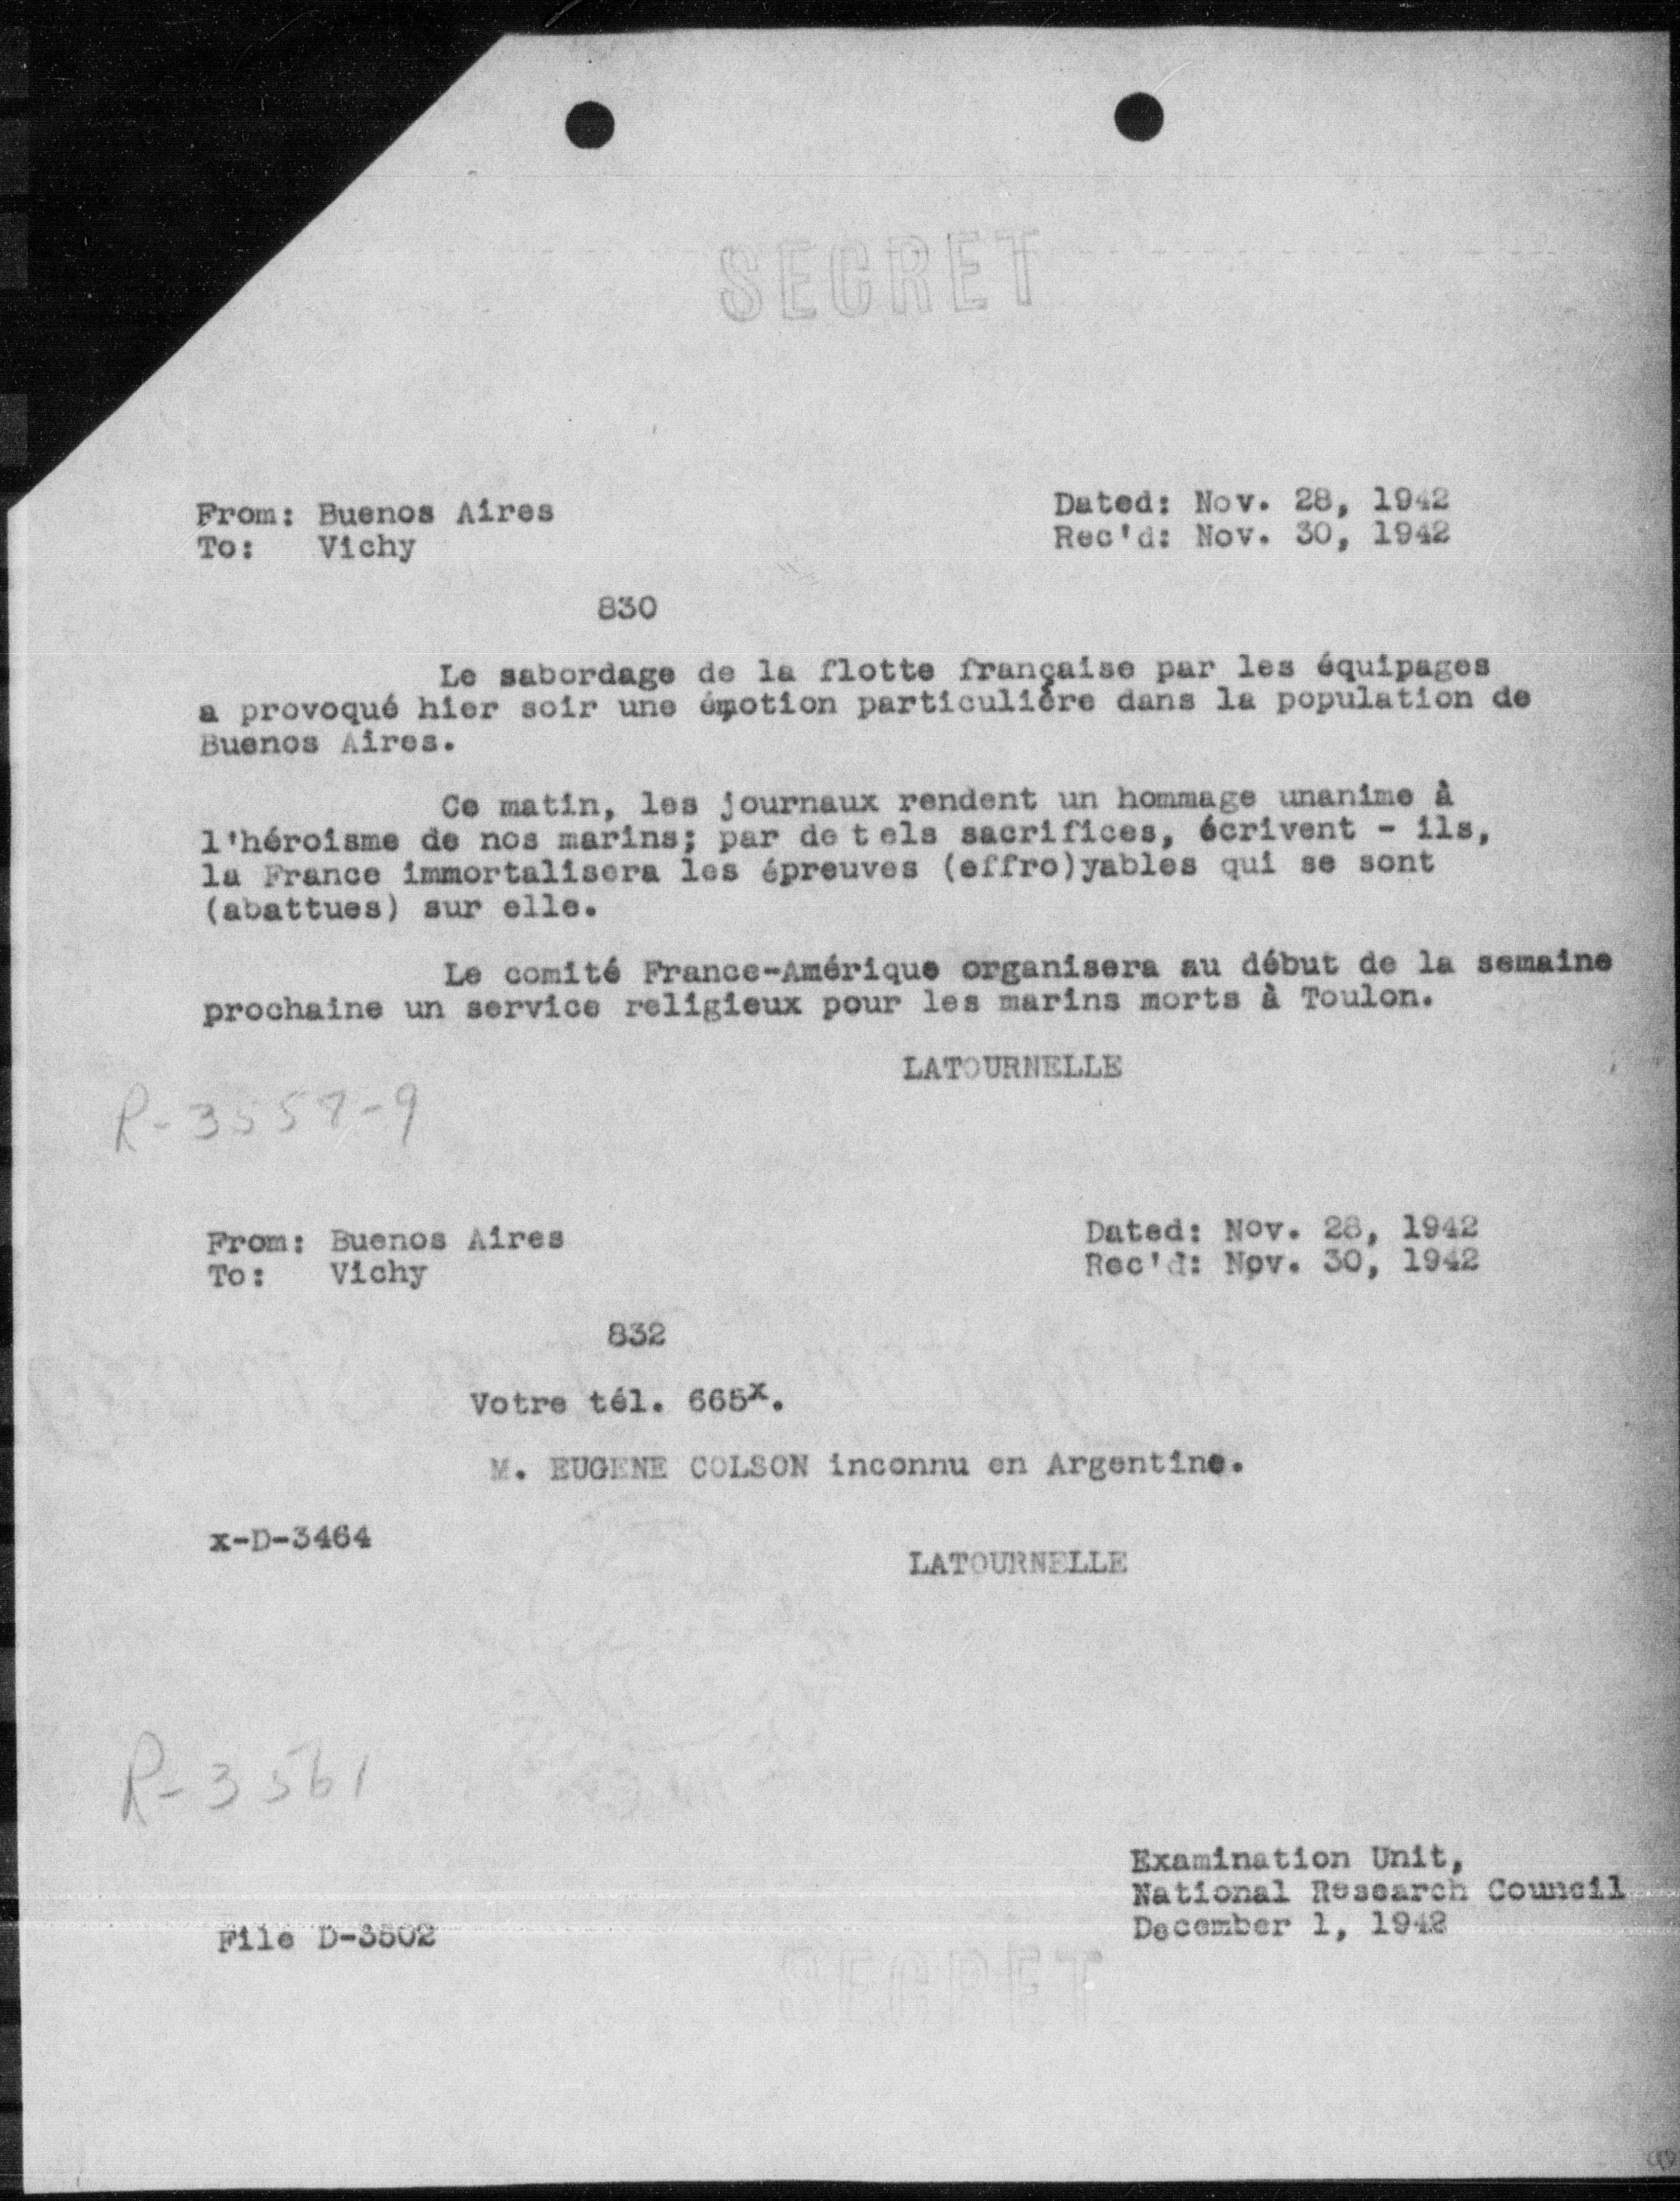
\includegraphics[width=\linewidth]{images/Reel 17428 - Page 2885.jpg}
    \caption{Image 2885 de la bobine T17428 (Canada Department of National Defence).}
    \label{fig:fig1}
    \vspace{-.3cm}
\end{wrapfigure}
Malgré cette accessibilité physique, l'absence de transcription ou de
métadonnées structurées rend le corpus difficilement inexploitable pour
des recherches ciblées ou pour l'utilisation de méthodes d'analyse
computationnelle. Ce verrou limite concrètement plusieurs lignes de
recherche historique dont la faisabilité dépend directement de la
cherchabilité du fonds, par exemple:

\textbf{Analyse des réseaux diplomatiques:} la quantification et la
cartographie des flux de communication entre les principaux postes
consulaires (Washington, Ottawa, Alger, Buenos Aires, Madrid, etc.) et
leur évolution au fil du conflit permettraient de reconstruire la
géographie relationnelle de la diplomatie vichyste, impossible à établir
par lecture manuelle sur un corpus de cette échelle en complément des
connaissances déjà construites.

\textbf{La rupture Vichy / France libre:} la transition d'octobre 1944
inscrite dans ce même fonds offre une opportunité comparative pour
analyser les continuités et ruptures dans les pratiques diplomatiques,
les réseaux de personnes et les thématiques entre les deux régimes.

\textbf{Recherche thématique ouverte:} un chercheur souhaitant étudier,
par exemple, la marine française et son implantation dans les colonies
des Antilles pendant le conflit peut, grâce à la cherchabilité du
corpus, identifier instantanément l'ensemble des télégrammes pertinents
par des requêtes booléennes --- une capacité fondamentale pour tout
travail monographique ou thématique s'appuyant entre autres sur ce
fonds.

Notre contribution présente la chaîne de traitement complet développé
pour lever ce verrou, en documentant ses résultats, ses limites et les
questions de soutenabilité qu'il soulève.

\section{Méthode: chaîne de traitement automatisée en cinq
phases}\label{muxe9thode-chauxeene-de-traitement-automatisuxe9e-en-cinq-phases}

\begin{figure}[htp]
    \vspace{-2cm}
    \centering
    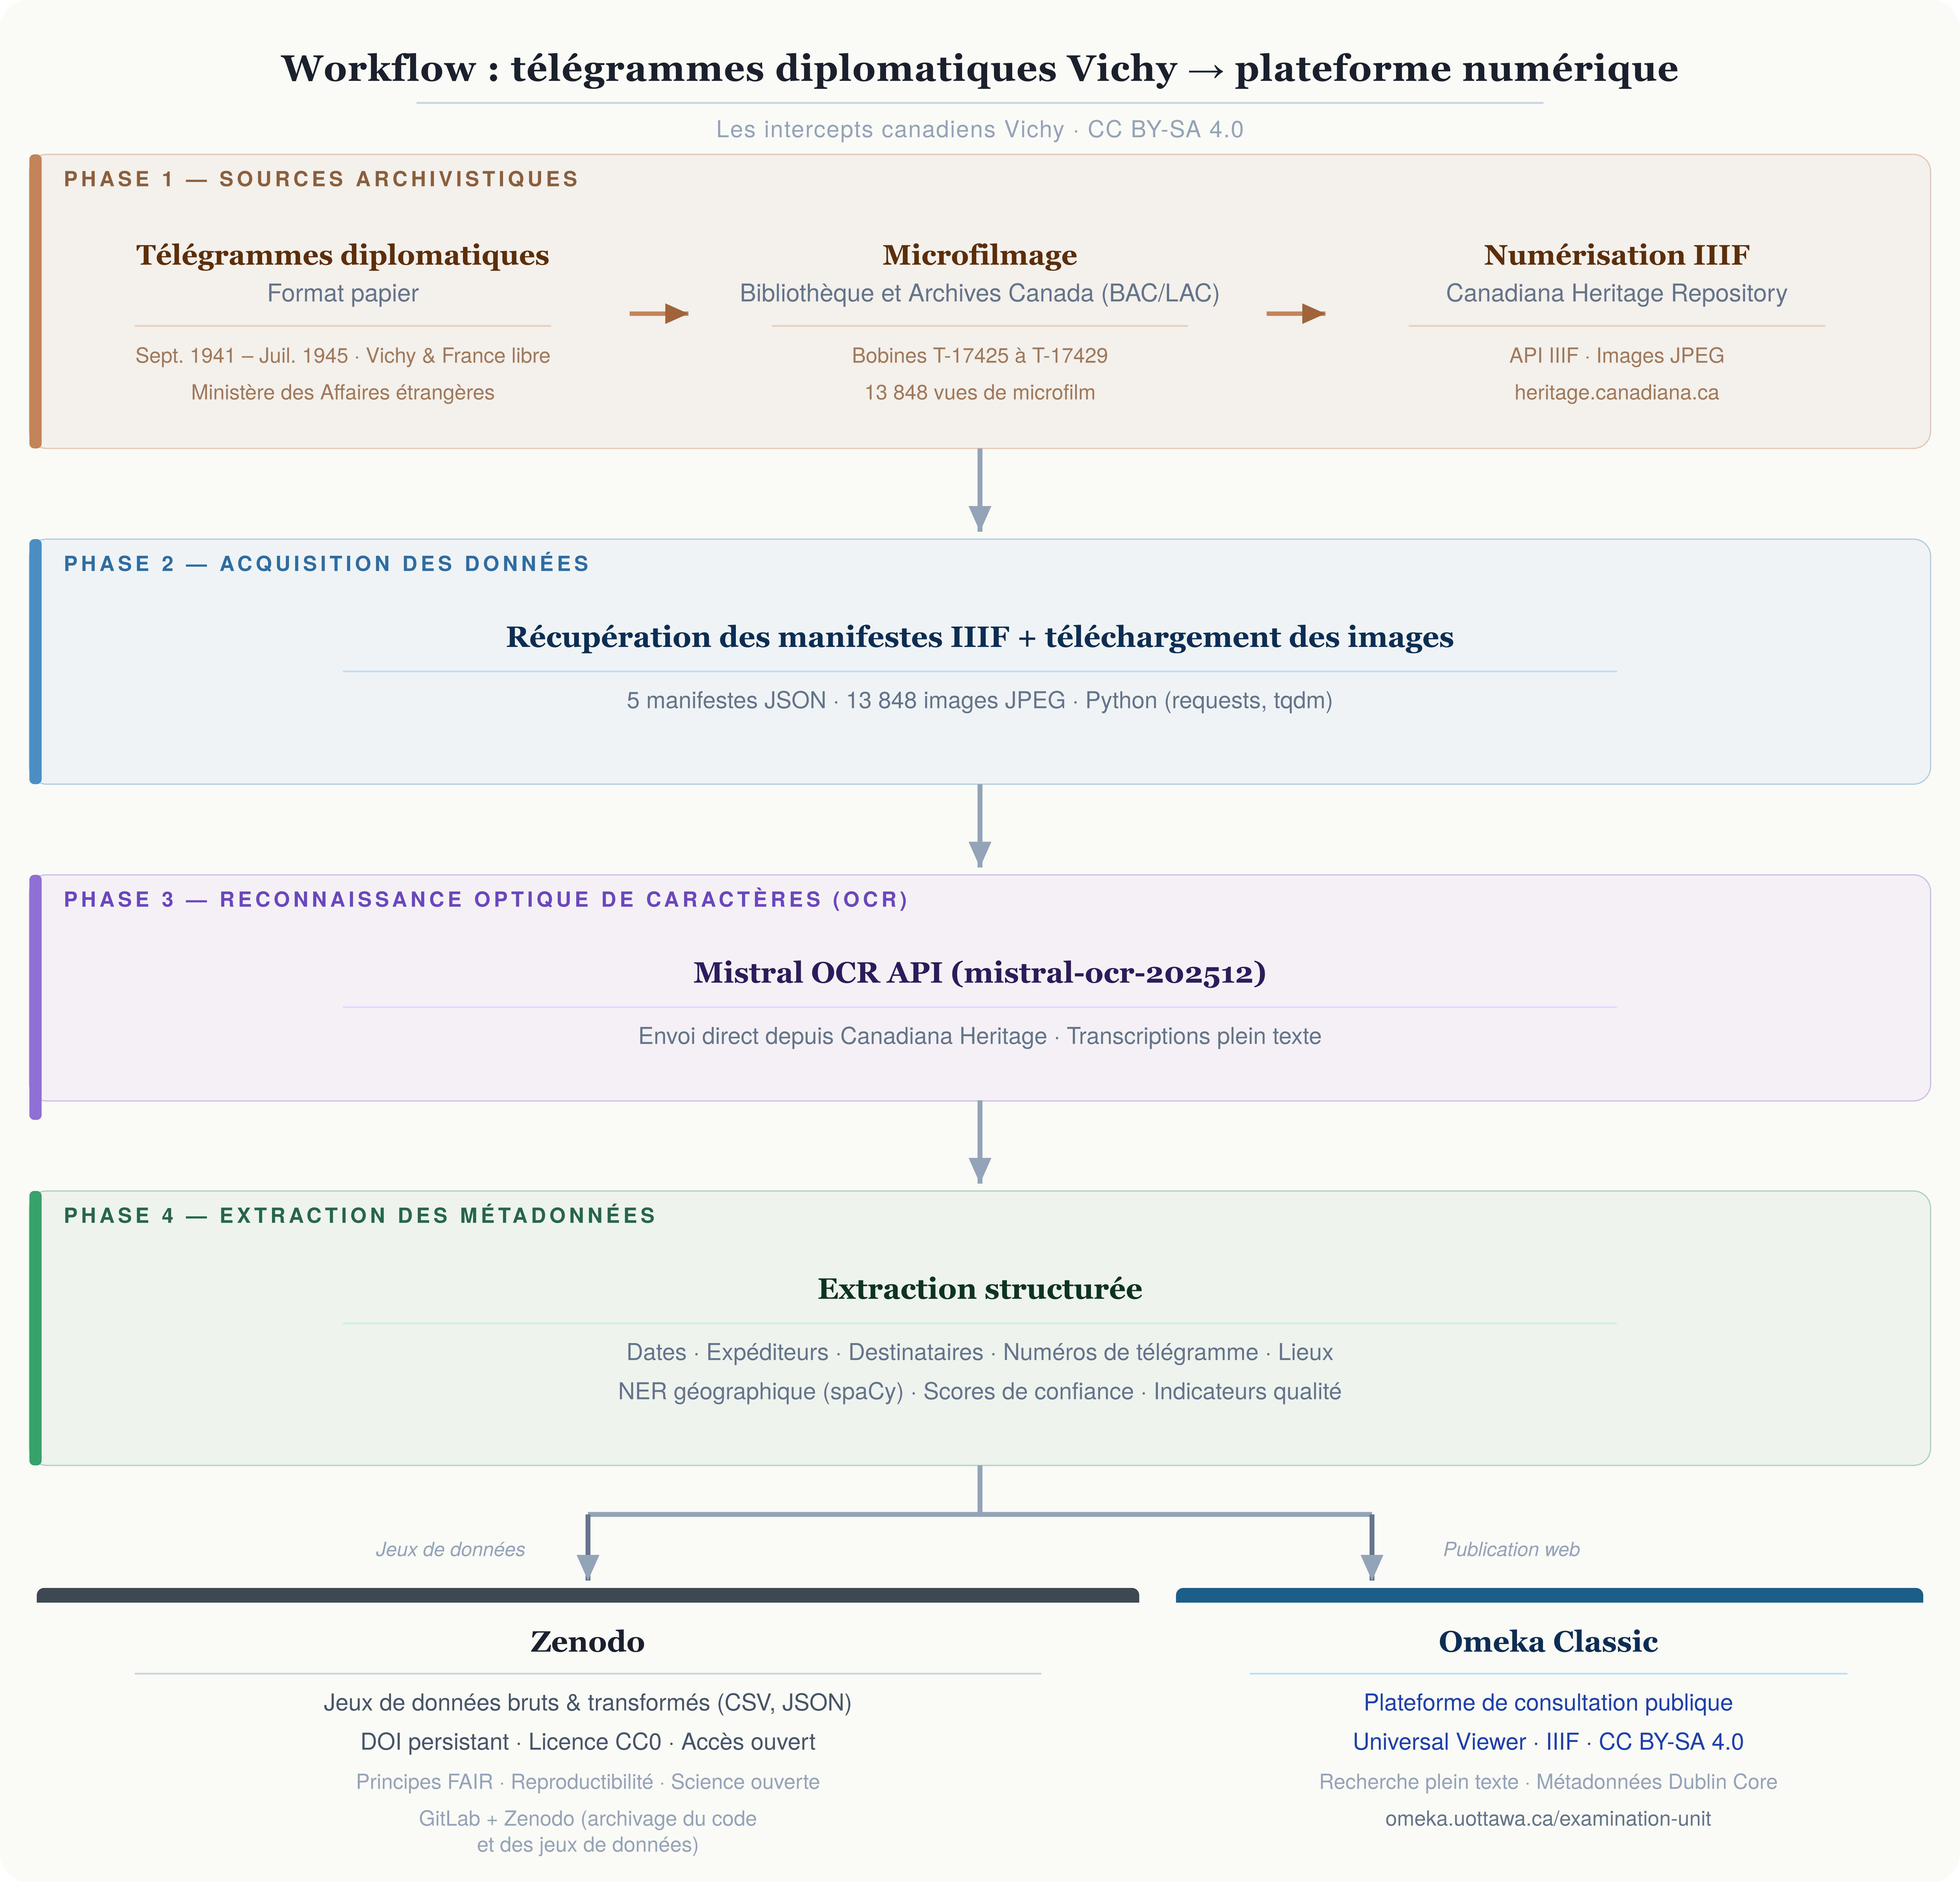
\includegraphics[width=.9\linewidth]{images/vichy_workflow_v1_1.png}
    \vspace{-.3cm}
    \caption{Flux de production du projet des images jusqu'à la mise à disposition.}
    \label{fig:flux}
    \vspace{-.5cm}
\end{figure}

Notre approche repose sur un flux de production reproductible schématisé
sur la Figure \ref{fig:flux}. Elle articule quatre phases distinctes, privilégiant
l'automatisation maximale, la documentation rigoureuse et l'utilisation
de formats ouverts. Les phases 1 et 2 du diagramme se sont pas listée
ici, car les télégrammes étaient déjà numérisés et accessibles, et les
images ont été téléchargées. Le développement et le traitement complet
du corpus se sont étendus sur trois mois, combinant développement
logiciel (Python 3.8+) et traitement à grande échelle.






\textbf{Phase 3 --- OCR par intelligence artificielle.} Les documents
présentent des défis techniques: frappe mécanique des années 1940
dégradée par plusieurs générations de microfilmage, mélange de français
et d'anglais, abréviations diplomatiques non standardisées et
annotations manuscrites marginales. Le choix s'est porté sur Mistral AI
(modèle \emph{mistral-ocr-2512}) \cite{mistralocr2026}, un modèle
multimodal optimisé notamment pour les documents historiques typewrités,
dont les performances sur ce type de corpus se sont révélées adaptées à
nos contraintes (voir la Figure~\ref{fig:fig1} et sa transcription \textit{infra}). Le traitement
complet a été effectué via l'API REST de Mistral OCR\footnote{\url{https://docs.mistral.ai/api/endpoint/ocr}.}
avec un système de traitement parallèle (cinq requêtes simultanées) et
gestion automatique des erreurs, pour une durée totale d'environ quinze
heures. Les résultats ont été stockés en deux formats complémentaires:
fichiers TXT pour l'interopérabilité et fichiers JSON incluant les
métadonnées techniques complètes.

\textbf{Phase 4 --- Extraction de métadonnées structurées.} Une chaîne
de traitement automatisée développée en Python transforme le texte brut
en métadonnées structurées exploitables. Le système détecte
automatiquement les frontières documentaires puis extrait les champs
essentiels: émetteurs, destinataires, dates d'envoi et de réception,
numéros de messages et signatures. Les techniques employées combinent
des expressions régulières optimisées, du \emph{fuzzy matching}
utilisant la distance de Levenshtein pour gérer les variations
orthographiques, et une base de données géographiques recensant plus de
150 lieux diplomatiques. Les résultats quantitatifs démontrent
l'efficacité de l'approche: environ 85\% des dates ont été
correctement extraites et normalisées au format ISO 8601\footnote{Ce
  nombre est une estimation temporaire, l'analyses étant encore en cours
  à la date de publication de cet article.}.



\textbf{Phase 5 --- Reconnaissance d'entités nommées.} Un module de
\emph{Named Entity Recognition} (NER) enrichit automatiquement le corpus
par l'extraction d'entités géographiques (villes, pays) et de personnels
diplomatiques. Cette couche d'annotation constitue le socle technique
des analyses de réseaux planifiées.

\textbf{Diffusion et préservation.} La collection est publiquement
accessible via une plateforme Omeka hébergée à l'Université
d'Ottawa\footnote{\url{https://omeka.uottawa.ca/examination-unit}.}.
L'interface offre une recherche plein texte sur l'ensemble du corpus,
des filtres par métadonnées et un accès aux images originales via
protocole IIIF. Des dépôts pérennes sur Zenodo ont été créés et seront
mis à jour au fil de l'évolution du projet. Ils incluent l'attribution
d'un DOI et l'attribution d'une licence CC BY-SA 4.0\footnote{Les dépôts
  du projet sont disponibles dans la communauté Zenodo créée
  spécifiquement à l'URL:
  \url{https://zenodo.org/communities/examination-unit} et le code du
  projet est sur la plateforme GitLab:
  \url{https://gitlab.com/untracked7957/examination-unit}.}.

  \begin{figure}[htp]
    \vspace{-.2cm}
    \begin{minted}[
    frame=lines,
    framesep=2mm,
    fontsize=\small,
    baselinestretch=1.2]
    {xml}
From: Buenos Aires
To: Vichy
Dated: Nov.~28, 1942
Rec'd: Nov.~30, 1942
830
Le sabordage de la flotte française par les équipages a provoqué hier
soir une émotion particulière dans la population de Buenos Aires.
Ce matin, les journaux rendent un hommage unanime à l'héroïsme de nos
marins; par de tels sacrifices, écrivent-ils, la France immortalisera
les épreuves (effro)yables qui se sont (abattues) sur elle.
Le comité France-Amérique organisera au début de la semaine prochaine un
service religieux pour les marins morts à Toulon.
LATOURNELLE
R-3559-9
From: Buenos Aires To: Vichy Dated: Nov.~28, 1942 Rec'd: Nov.~30, 1942
832 Votre tél. 665K.
M. EUGENE COLSON inconnu en Argentine.
x-D-3464 LATOURNELLE
R-3561
File D-3502 Examination Unit, National Research Council December 1,
1942
    \end{minted}
    \vspace{-.4cm}
    \caption{Transcription brute après OCR de l’image du télégramme de la Figure~\ref{fig:fig1}.}
    \label{fig:telegramme}
    \vspace{-.4cm}
\end{figure}

\section{Résultats: un corpus structuré et
accessible}\label{ruxe9sultats-un-corpus-structuruxe9-et-accessible}

La chaîne de traitement a transformé les 13 848 pages en un corpus
numérique structuré et interrogeable. L'extraction automatisée est en cours de finalisation et a permis d'identifier environ 11 000 télégrammes distincts. Les métriques d'extraction
temporaires reflètent à la fois l'efficacité de la chaîne de traitement
et les défis propres à ce type de documents: 75\% de réussite pour
l'extraction des dates d'envoi, 51\% pour les numéros de messages et 86\%
des postes émetteurs et récepteurs. Ces performances restent
confrontées à plusieurs défis documentés: fragmentation des métadonnées
sur les documents multipages, variations orthographiques des noms de
lieux, et ambiguïtés entre dates d'envoi, de réception et de décodage.

La valeur concrète du corpus cherchable se mesure directement à travers
des cas d'usage. Par exemple, un chercheur souhaitant étudier la marine française et
son implantation aux Antilles pendant le conflit peut, via l'interface
Omeka, interroger l'intégralité du corpus par requêtes
booléennes et identifier instantanément les documents pertinents -- une
opération qui aurait nécessité la lecture exhaustive de milliers de
pages dans le format image original\footnote{Exemple de requête
  permettant une recherche booléenne sur les Antilles:
  \href{https://omeka.uottawa.ca/examination-unit/search?query=guadel*+OR+caraib*+OR+antill*+OR+martiniq*+OR+\%22Fort-de-France\%22+OR+\%22Port-de-France\%22&query_type=boolean&record_types\%5B\%5D=Item&record_types\%5B\%5D=File&record_types\%5B\%5D=Collection&record_types\%5B\%5D=Exhibit&record_types\%5B\%5D=ExhibitPage&record_types\%5B\%5D=SimplePagesPage&submit_search=Submit}{\url{https://omeka.uottawa.ca}}.}.
Cette capacité de recherche thématique ouverte constitue la contribution
opérationnelle centrale du projet pour la communauté des historiens.

La transparence constitue un principe directeur: les erreurs connues
sont explicitement signalées, les images originales demeurent
accessibles pour vérification, et les données sont exportables aux
formats CSV et JSON pour réutilisation computationnelle. L'accès est
gratuit et sans inscription, conformément aux principes de science
ouverte.

\section{Discussion: arbitrages techniques et questions de
soutenabilité}\label{discussion-arbitrages-techniques-et-questions-de-soutenabilituxe9}

La transformation de ce corpus confronte à un trilemme méthodologique
dont les implications environnementales varient considérablement selon
le scénario retenu. Le statu quo -- maintenir uniquement les images
haute résolution -- présente un impact environnemental direct quasi
nul, mais perpétue l'inaccessibilité computationnelle et rend
impossibles les analyses historiques dont des exemples sont fournis plus
haut. La transcription manuelle intégrale garantirait une haute qualité
avec un impact environnemental estimé à 120--810 kWh, mais les 3 000-4
500 heures de travail humain nécessaires\footnote{Cette fourchette
  repose sur une vitesse de transcription manuelle soigneuse estimée
  entre 3 et 4,5 pages/heure pour ces documents dactylographiés. À 3
  pages/heure (hypothèse conservatrice), 13 848 pages représentent
  environ 4 616 heures ; à 4,5 pages/heure (hypothèse optimiste),
  environ 3 077 heures. Sur le plan énergétique, la consommation directe
  du poste de travail a été estimée selon trois scénarios. Appliquée à
  la fourchette de 3 000--4 500 heures, cette hypothèse produit une
  plage de consommation électrique directe de 120 à 810 kWh.} la rendent
économiquement irréaliste sans financement majeur. L'OCR par
intelligence artificielle, option retenue, combine environ 120 heures de
travail humain avec un coût computationnel d'inférence GPU dont l'impact
environnemental reste à quantifier précisément -- une évaluation
systématique (13 848 requêtes API, infrastructure GPU de Mistral AI) est
en cours et fera l'objet d'une publication ultérieure incluant également
une évaluation de l'impact social du projet.

Ce coût ponctuel peut notamment être justifié par une perspective de
science ouverte: en rendant les données immédiatement disponibles et
réutilisables sous licence CC BY-SA 4.0, nous évitons que d'autres
chercheurs ne reproduisent ce traitement, amortissant ainsi l'empreinte
environnementale initiale. Cette mitigation par mutualisation reste
elle-même à quantifier: combien de chercheurs réutiliseront
effectivement ces données, et sur quelle durée ? La science ouverte
constitue une condition nécessaire, mais probablement insuffisante pour
justifier l'usage de l'IA sans mesures d'impact précises.

Ce projet adopte donc une posture de documentation expérimentale plutôt
que de validation d'une solution optimale. La question centrale demeure
ouverte: dans quels contextes, à quelles conditions et à quel coût
environnemental l'usage de l'intelligence artificielle devient-il
défendable pour la transformation d'archives patrimoniales? Ce corpus,
par la singularité historique des sources qu'il rend accessibles,
constitue un cas d'usage où l'enjeu scientifique semble suffisant pour
engager sérieusement ce débat. Plus généralement, la question de
l'impact environnemental de la numérisation d'un corpus donné invite
également au dialogue avec les études menées à des échelles plus
importantes telle qu'une unité de recherche \cite{CNRS_empreinte_2026}, 
voire d'une discipline entière sur le plan international \cite{knoedlseder_secnarios_2024}.

\section{Perspectives}\label{perspectives}

Le résultat immédiat du projet est un corpus de plus de 11 000
télégrammes diplomatiques désormais cherchables, structurés et librement
accessibles -- une ressource qui n'existait pas il y a 6~mois. Cette
disponibilité constitue en elle-même la contribution centrale: tout
chercheur travaillant sur la diplomatie française de la Seconde Guerre
mondiale, sur le renseignement canadien, ou sur des thématiques connexes
peut dès aujourd'hui interroger ce fonds selon ses propres questions de
recherche, sans avoir à reproduire le traitement.

Des approches méthodologiques moins traditionnelles peuvent également
être utilisées, comme par exemple l'analyse des réseaux diplomatiques
tel que l'ont fait certains chercheurs par le passé \cite{bloch_networks_2022,jo_diplomatic_2016}.
La perspective principale est donc moins de prescrire un programme
analytique que de catalyser une communauté de chercheurs qui
s'appropriera ces données et la plateforme selon des angles que le
projet lui-même n'a pas anticipés.

L'amélioration continue du corpus repose sur une dimension collaborative
structurée. La plateforme Omeka pourrait servir de support à une
correction \emph{crowdsourcée} de l'OCR, à la validation des métadonnées
par des experts de l'histoire de Vichy, et à l'ajout d'annotations
thématiques. Cette stratégie participative offre également une voie vers
des arbitrages technologiques plus soutenables: l'expérience acquise
suggère qu'une approche alternative privilégiant des modèles OCR
\emph{open source} sur CPU, dont les imperfections seraient
progressivement compensées par la communauté, pourrait constituer un
modèle plus équilibré pour des projets futurs similaires.

\nocite{bloch_networks_2022,}
\nocite{dpt_national_defence}
\nocite{eberlee_scholar_2024}
\nocite{CNRS_empreinte_2026}
\nocite{examination_textual_record}
\nocite{hawkins_archives_2022}
\nocite{jensen_cautious_2008}
\nocite{jo_diplomatic_2016}
\nocite{knoedlseder_secnarios_2024}
\nocite{mistralocr2026}
\nocite{wesley_cryptographic_1987}
\printbibliography


\end{document}
